\chapter{Implementierung}\label{implementation}

In diesem Kapitel wird der Vorgang der Implementierung des digitalen Prototypen erläutert. Zunächst wird ein kurzer Einblick über die verwendete Spiele Enigen Unity gegeben und wichtige Komponente erklärt. 
Anschließend wird die Auswahl der Traking Framework sowie die verwendete Traking Methode erläutert. Es wird die Wahl der passenden Zeige und Auswahl Methode erläutert sowie die Verarbeitung der 
Eingabedaten über die Touchscreen Oberfläche an mit einer Flussdiagramm veranschaulicht. Abschließend wird er digitale Prototyp vorgestellt und die Vorbereitung des Prototypen auf die Studie erklärt. 

\section{Entwicklungsumgebung}

\subsection{Game Engine}

Unity ist ein Spieleengine des Unternehmens Unity Technologies und stellt eine Entwicklungsumgebung vorwiegend für Spiele dar. Jedoch hat sich Unity seither 
zu einem vielseitigen Werkzeug auch in anderen Bereichen als der Spieleenwticklung (z. B. im Bereich der Industrie) entwickelt. 
Unity ermöglicht die Entiwcklung von Anwendung für über 25 Plattformen darunter Plattformen für mobile Endgeräte wie Android oder iOS.

Zu den für die Verständnis dieser Arbeit wichtigen Komponente der Unity Umgebung zählen Szenen, Komponente, Prefabs sowie GameObjekts. Folgend werden diese kurz erläutert:

\textit{Szenen:} In Unity ist die Entwicklung in Szenen organisiert. Jede Szene besteht aus einem Szenengraph. Dieser Graph enthält wiederum weiter Objekte wie z. B. Game Objekte. 

\textit{GameObejects:} Game Objekte stellen in Unity Objekte dar wie zum Beipsiel eine Lichtquelle, eine Audioquelle oder eine geometrische Form wie ein Würfel. Game Objekte erhalten Eigenschaften durch 
Hinzufügen von Komponente. \cite{Unity}\\

\textit{Komponente:} Komponente geben Game Obejekten Eigenschaften und steuern diese. Eine Komponente kann zum Beispiel ein Material sein welches gewisse Eigenschaften wie eine Farbe oder Textur hat. 
Durch das hinzufügen eines Skriptes als Komponente an ein Game Objekt kann dieses darüber gesteuert werden.\cite{Unity}\\

\textit{Prefabs:} In Unity können Game Obejekte vorgefertigt sodass diese nicht zur Laufzeit erstellt werden müssen. Dies vorgefertigten Game Objekte sind so genannte Prefabs welche. Es kann zur Laufzeit eine Instanz eines Prefabs erzeugt werden.\cite{Unity}\\

Zu den unterstützten Programmiersprachen in Unity zählen Java Script und C\#. Für die Entwicklung des digitalen Prototypen wird die Programmiersprache C\# verwendet und die Visual Studio IDE der Firma Microsoft genutzt. 

\subsection{Tracking}

% Am besten geeignet: Kombination aus Modellbasiertes Tracking mit Verwendung eines CAD Modell des Produktes und Modellfreis Tracking damit das Traking aufrecht erhalten bleibt auch wenn nur Teile des Produktes im Sichtbereich der Kamera ist. 
% Ausprobiert wurde Model Tracking mit Vuforia sowie VisionLib. Vuforia hat nicht geklappt. VisionLib hat sehr gut geklappt mit Testlizez am Beispiel Model. Mit unterschiedlicher Beleuchtung, mit Bewegung des Models. 
% Jedoch war Lizenzverlängerung nicht möglich da Lizenztool für die Generierung von Lizenzen zur akademischen Nutzung nur für IOS möglich war. 

Da die Applikation verwendet werden soll um Produkte mit virtuellen Informationen war es naheliegend ein Traking Verfahren zu wählen welches für die Registrierung die Produkte selbst nutzen kann: Modellbasiertes Tracking mit Verwendung von 3D CAD Modell des Produktes. 
Hierzu wurden zwei Framework in Betracht gezogen und ausprobiert. Das AR Tracking Framework der Vuforia der Firma PTC sowie VisionLib der Firma Visometry GmbH. 

Zu dem Vorteilen von Vuforia zählten, dass Vuforia als Framework in Unity bereits integriert ist sowie die Ermöglichung eine Kombination von modellbasieten und modellfreies Tracking zu verwenden. 
Mit Vufofia kann wahlweise für modellfreies Tracking die Frameworks ARCore für Android Endgeräte oder ARKit für iOS Endgeräte verwendet werden. 

Auf der anderen Seite waren die Vorteile des VisionLib Framework die dass dieses, sich durch eine schlanke SDK schnell in Unity integrieren lässt. Zudem erschien das Tracking von 3D Modellen mit VisionLib stabil und wenig empfindlich gegen 
unterschiedlichen Lichtverhältnissen, Bewegungen des Modells sowie z. B. geringer Textur des Modells zu sein. \footnote{Beschreibung des VisionLib Framework: https://visionlib.com/awe/ [Letzter Zugriff: 07.09.2019]}

Das Tracking mit dem VisionLib Framework wurde am Beispiel eines vom Hersteller bereitgestellten Spielzeugauto aus Papier getestet. Nach einer Kalibrierung der Kamera konnte das Tracking getestet werden. Das Spielzeugauto wurde mit unterschiedlichen
Lichtverhältnisse (Tageslicht, Abends bei gedimmten Licht) sowie mit mäßiger Bewegung des Modells getestet. Bei schneller Bewegung der Kamera oder des Modells konnte das ging kam ging die Registrierung verloren jedoch erschien das Tracking im allgemeinen sehr stabil.
Unterschiedliche Lichtverhältnisse haben nur geringen Einfluss auf die Qualität des Trakings gehabt. Leider konnte das VisionLib Framework für ein Test an einem größeren Model nicht weiter genutzt werden da die beantragte Testlizenz bereits abgelaufen war. Vom Hersteller wurde die akademische Nutzung ein Lizenz angeboten, es konnte jedoch mit dem Lizenzgenerierungs-Tool dieser Liezenzen nur Lizenzen für iOS Endgeräte erzeugt werden. 

Für die Nutzung von 3D Modellen zur Objekterkennung in Vuforia konnte das vom Hersteller zur Verfügung gestellte Tool Model Target Generator verwendet werden. In diesem konnte ein 3D CAD Model des Produktes geladen werden und ein Binärdatei erzeugt werden welches 
in Unity geladen werden kann. Das Tracking wurde am Beispiel eines Autos ausprobiert hat jedoch nicht geklappt. Die Ursache dafür lag vermutlich daran dass das Modell zu aus zu vielen Polygonen bestand (über 600.000). Laut dem Hersteller kann das müssen Modelle mit mehr als 400.000 Polygonen für 
ein erfolgreiches Tracking vereinfacht werden. 

Zuletzt wurde beschlossen mit Verwendung von Vuforia als Tracking Framework ein Bild mit natürlichen Bildmerkmalen, ein sogenanntes Image Target in Kombination mit ein modellfreies Verfahren zu verwenden.


\section{Verarbeitung der Eingabedaten}

% Vertikal. Wurde zuerst Crossfade entwickelt und von Nutzern getestet. War blöd.. haben intuitiv Bildschirm berürht zum auswählen. Zudem war blöd dass für das Auswählen der Blick von Auswahlstelle zum Button gewächslt werden musste während Handy in der position zum auswählen gehalten werden musste. 
% geändert zum relativ pointing. 
% bestätigung auftauchen des Buttons an der Stelle wo geklikt wurde. Bleibt eine bestimmte Zeit und verschwindet falls keine eingabe oder neues zeigen. 
% Problem mit Szenenwächsel. AR Cameara. Workaround. 

%Flow diagramm

Wie im Kapitel zuvor beschrieben wurde beschlossen für das Zeigen auf dem Produkt und dem Auswählen von Produktteile zwei unterschiedliche Methoden als vertikale Prototypen zu entwickeln und von einer kleinen Gruppe an Testnutzern ausprobieren zu lassen. 
Zunächst wurde die Methode \textit{Crossfade} implementiert. Abbildung \ref{fig:crossfade_create} zeigt das Auswählen eins Produktteil oder Stelle. In der Mitte des Bildschirmes dient der Fadenkreuz zum Anvisieren auf dem Produkt. Es wird ein Ray ausgehend von der 
Kamera in die Welt ausstrahlt. Trifft dieses ein Produktteil erschient im unteren Rand des Bildschirms ein Button zum auswählen dieser Stelle. Beim klicken auf diesen Button wurde zu diesem Zeitpunkt der Entwicklung zunächst nur ein Würfel auf die ausgewählte Stelle platziert.
Abbildung \ref{fig:crossfade_edit_delete} zeigt den Vorgang für das Editieren oder Löschen. Wurde die Kamera auf ein Würfel gerichtet, welche in diesem Stand der Entwicklung zunächst durch Würfel repräsentiert wurden, ersschienen am unteren Rand des Bildschirmes zwei Buttons zum editieren oder löschen. 

\begin{figure}[H]
	\label{tab:example}
	\centering
	\begin{minipage}{.4\textwidth}
		\centering
		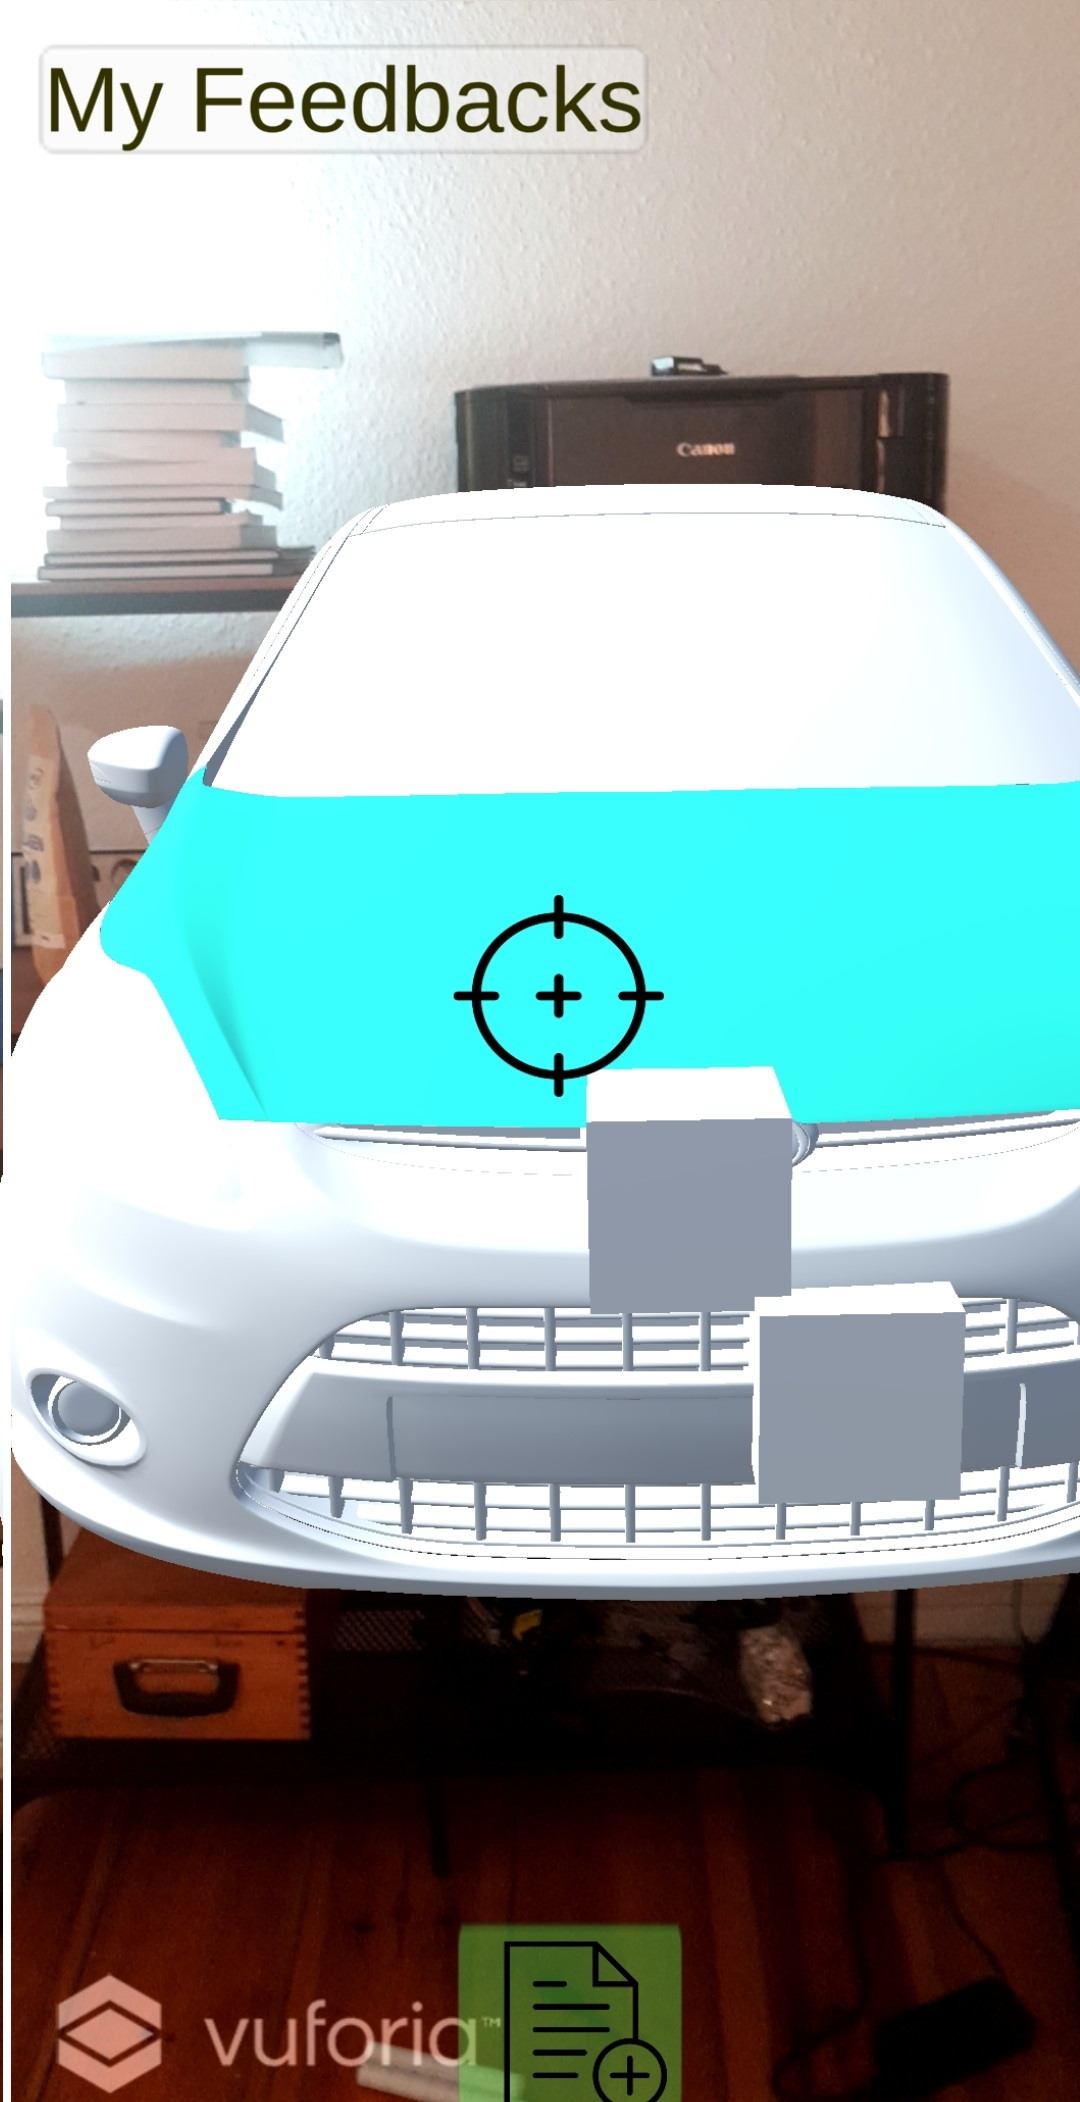
\includegraphics[width=.65\linewidth]{resources/implementation/crossfade_create.jpg}
		\captionof{figure}{Digitaler Protottyp \\ Crossfade Methode Erstellen\\Quelle: Eigene Darstellung}
		\label{fig:crossfade_create}
	\end{minipage}%
	\begin{minipage}{.4\textwidth}
		\centering
		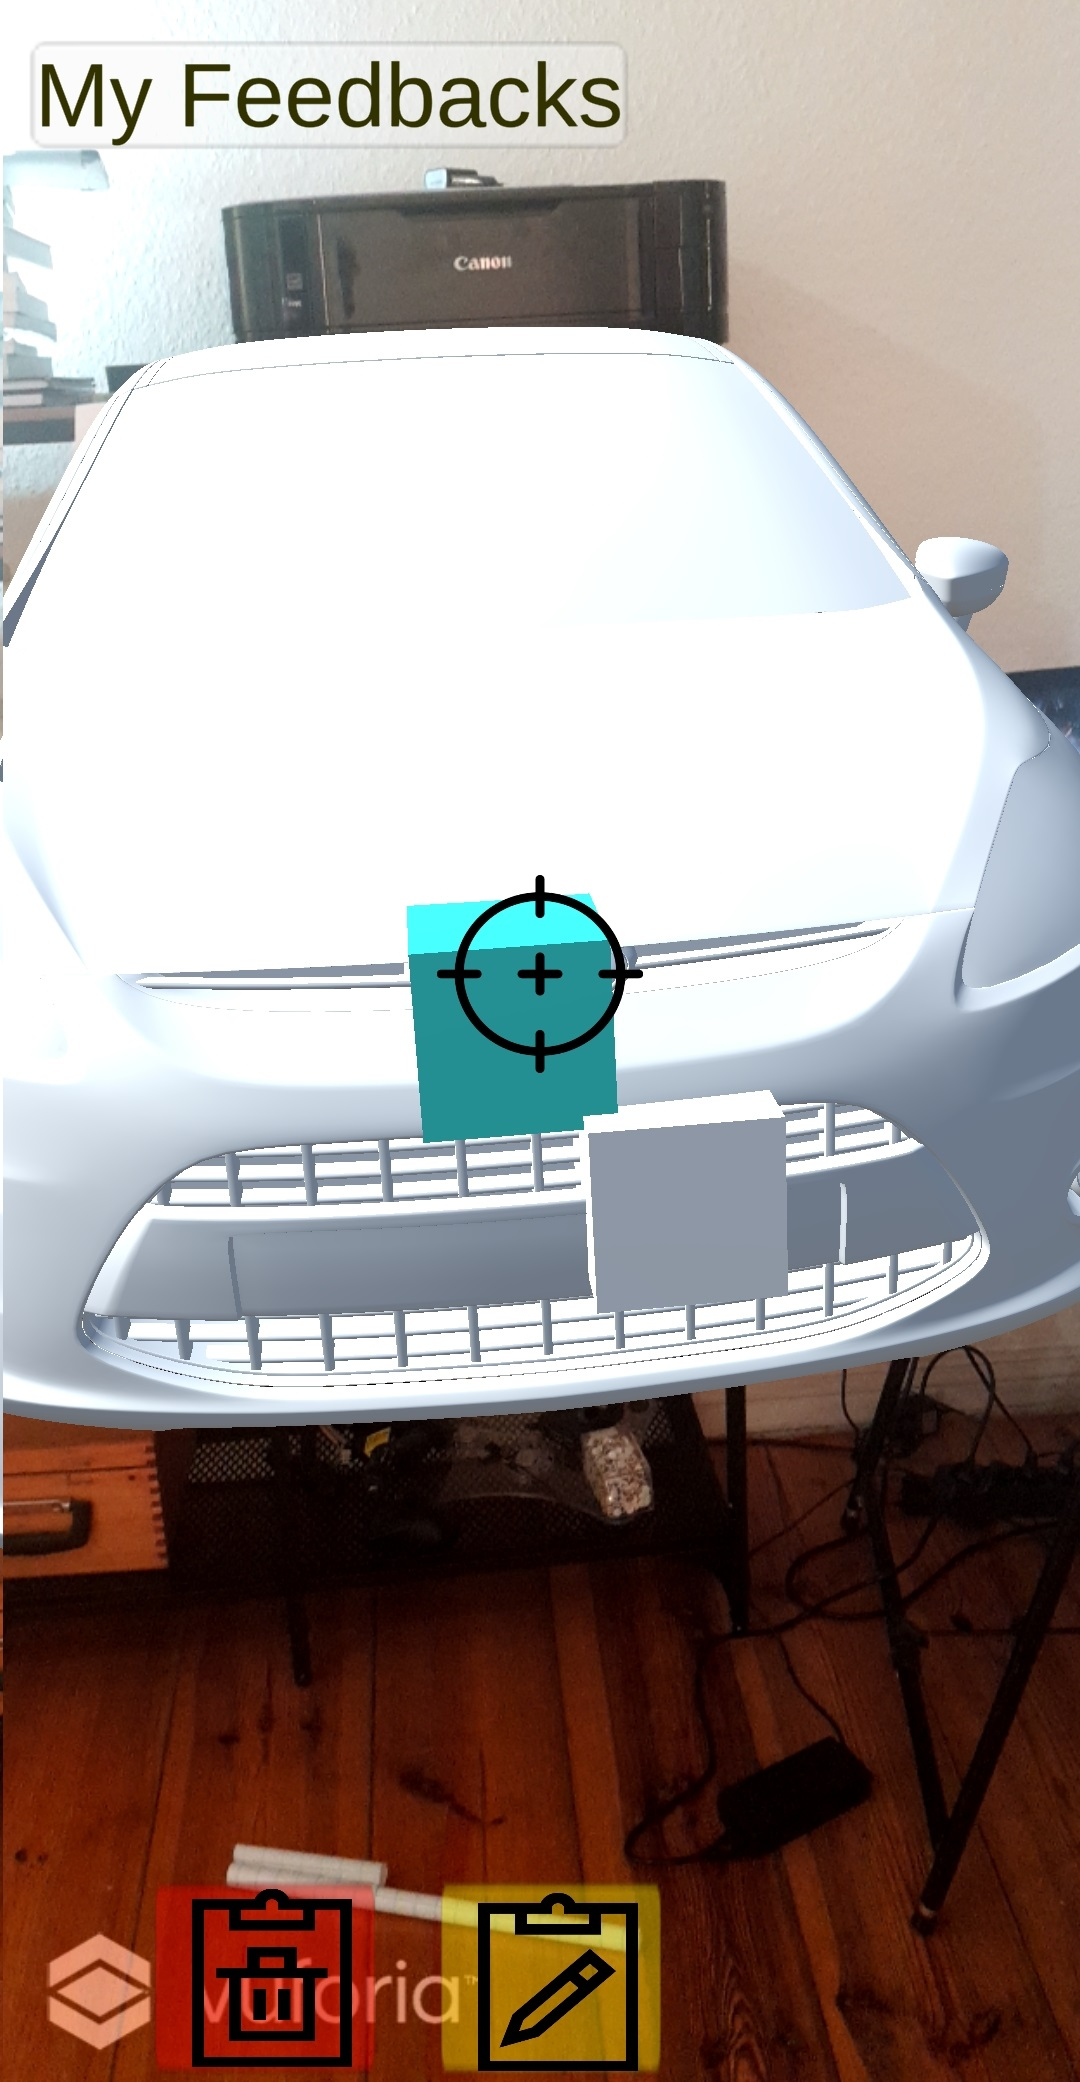
\includegraphics[width=.65\linewidth]{resources/implementation/crossfade_edit.jpg}
		\captionof{figure}{Digitaler Protottyp \\ Crossfade Methode Bearbeiten/ Löschen\\Quelle: Eigene Darstellung}
		\label{fig:crossfade_edit_delete}
	\end{minipage}
\end{figure}

Diese Methode wurde von vier Testnutzern getestet und als zu umständlich empfunden worden. Was bei der Nutzung aller Testnutzer beobachtet werden konnte, dass diese intuitiv auf eine beliebige Stelle oder auf den Fadenkreuz auf dem Bildschirm 
getippt haben und sehr spät gemerkt haben das sich am unteren Rand des Bildschirm ein Button zum Anlegen befindet. Die Anmerkungen der Nutzer zu dieser Variante waren, dass sie intuitiv angenommen haben dass sie auf das Bildschirm klicken oder wischen 
müssten um eine Stelle auf dem Produkt auszuwählen. Dies könnte sich dadurch erklären dass eine gewisse Erwartungskonformität durch die Nutzung von Touchscreen Oberflächen vorhanden ist. Zudem gab es die Anmerkung dass es recht Umständlich sei die Stelle 
am Produkt anvisiert zu lassen und gleichzeitig die Aufmerksamkeit auf das Button zum auswählen zu richten. Das zittern der Hände würde diesen Umstand weiter verschlimmern. 

So wurde entschieden mit der Implementierung der \textit{Relativ Pointing} Methode für das Zeigen und Auswählen auf dem Produkt fortzufahren.  Die Informationsverarbeitung während der Nutzung der Touchscreen Oberfläche für das Zeigen und Auswählen einer 
Stelle oder eines bereits existierenden Feedback veranschaulicht das Flussdiagramm auf Abbildung \ref{img:flow}. 

Die Interaktion mit der \textit{Relativ Pointing} Methode wurde wie folgt umgesetzt. 

Während des gesamten Vorangs wird ein Ray-Cast durchgeführt. Die Interaktion ist in drei Phasen aufgeteilt, die Phase in welcher der Finger auf das Bildschirm angelegt wird, die Phase in welcher der Finger auf dem Touch Bildschirm bewegt wird und die Phase in dem 
der Finger angehoben wird. Es wird ein Strahl ausgehend vom Position des Fingers auf dem Bildschirm, in die Welt hinein gesendet. 

Folgend sind die Interaktion Schritte beschrieben:

\begin{enumerate}
	\item Der Nutzer legt sein Finger auf das Touchscreen an. Dies ist der Startposition für das Zeigen. 
	\begin{enumerate}
	\item Es wird zunächst überprüft ob der Strahl ein bereits vorhandenes Feedback getroffen hat. Ist dies der Fall wird auf die aktuelle Position des Fingers ein zwei Buttons zum Editieren oder Löschen des Feedback platziert. Diese Buttons bleiben für eine bestimmte Zeit eingeblendet (z. B. 4 Sekunden) und werden ausgeblendet entweder wenn die Zeit abgelaufen ist oder wenn der Finger erneut an das Bildschirm an eine andere Stelle angelegt wird. 
	\item Falls der Finger einen Bereich auf dem Produkt trifft, werden alle auf dem Produkt vorhandenen Feedback ausgeblendet damit während des Auswahlvorgangs keine Bereiche auf dem Produkt verdeckt werden. Der Zeiger welches durch eine rote Kugel repräsentiert wird, wird an der Stelle die der Strahl auf dem Produkt getroffen hat platziert.
	\end{enumerate} 
	\item Der Nutzer bewegt sein Finger auf dem Touch Bildschirm.
	\begin{enumerate}
		\item Es wird überprüft ob ein Produktteil bereits Blau eingefärbt und so in Fokus gerückt ist. Ist dies der Fall, wird das eingefärbter Teil in die Standardfarbe gefärbt sodass dieser nicht mehr hervorgehoben wird und das Teil welches vom ausgesendeten Strahl getroffen wird wird in Blau eingefärbt.
		\item Ist auf dem Produkt ein Teil bereits in den Fokus gerückt. Wird das Teil welches vom Strahl getroffen wird Blau eingefärbt.  
		\item Der Zeiger wird auf dem Produkt in jeder Frame in welcher der Finger in Bewegung ist auf die Stelle auf dem Produkt gesetzt die der ausgesendete Strahl trifft.
	\end{enumerate} 
	\item Der Nutzer hebt sein Finger vom Bildschirm ab. Es werden alle vorhanden Feedback wieder auf dem Produkt eingeblendet. Es wir ein Button zum auswählen der Stelle auf dem sich aktuell der Zeiger auf dem Produkt befindet auf der Stelle auf dem der Finger des Nutzers beim anheben des Fingers auf dem Bildschirm befand eingeblendet.
\end{enumerate} 

Diese Methode wurde ebenfalls von Test Nutzern (darunter auch eine Nutzerin welche die \textit{Crossfade} Methode nicht getestet hatte) getestet und Iterationsschritte schnell verstanden. 

\begin{figure}[H]
	\centering
	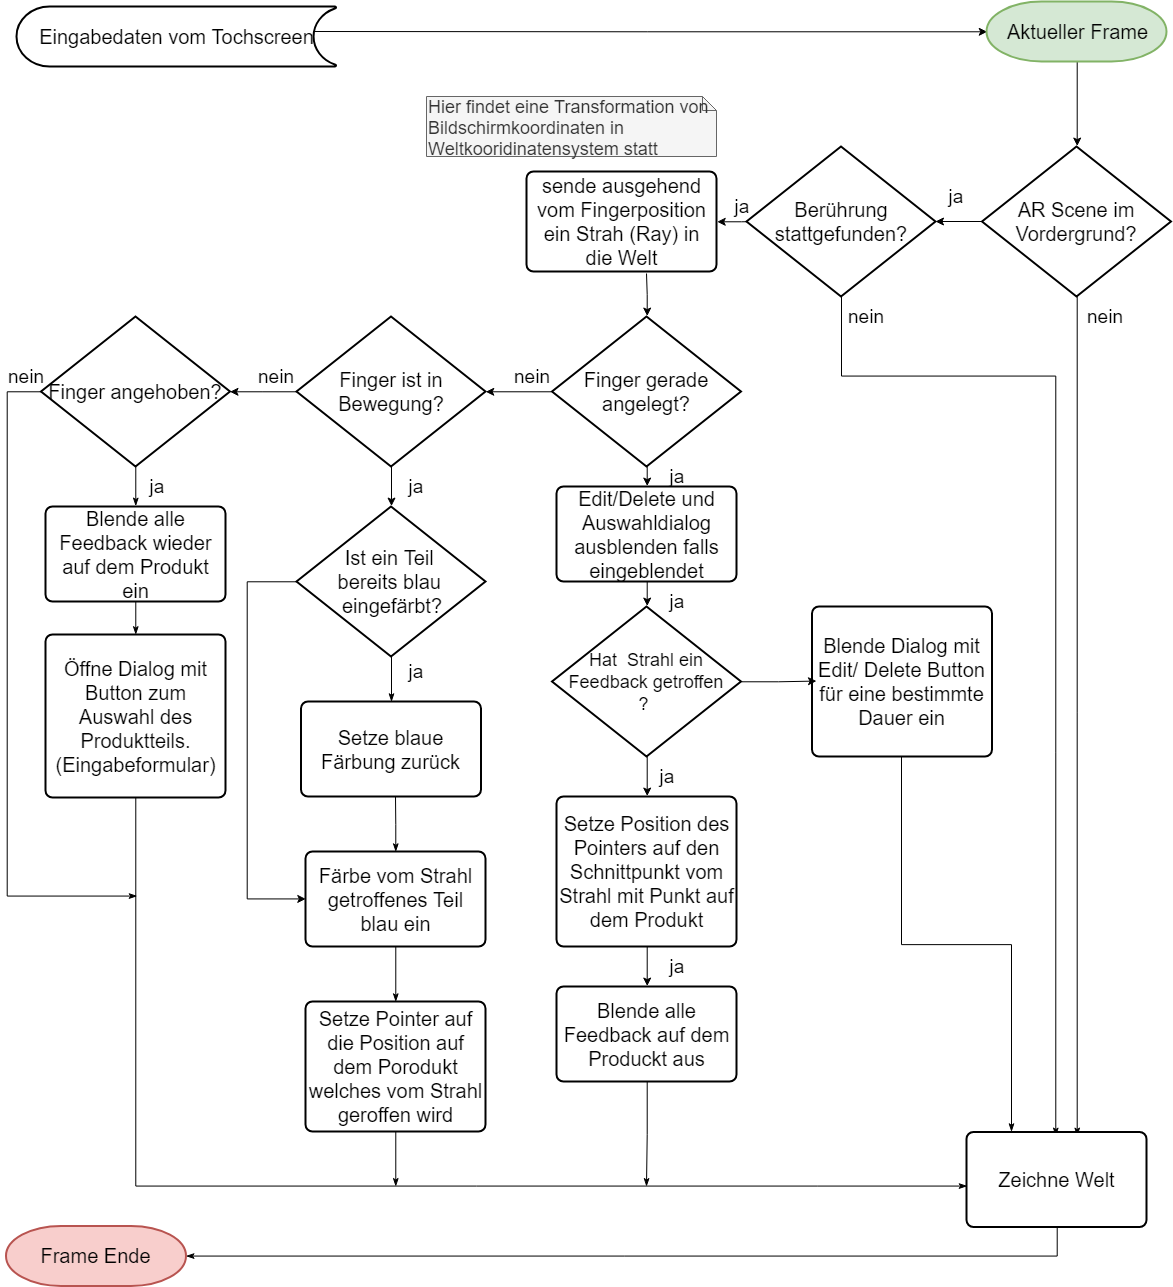
\includegraphics[width=1.0\textwidth]{resources/implementation/flussdiagram_selection.png}
	\caption{Flussdiagramm - Verarbeitung des Touchscreen Berührvorgang \\Quelle: Eigene Darstellung}
	\label{img:flow}
\end{figure}

\section{Vorstellung des digitalen Prototypen}

Im Folgenden wird der digitale Prototyp vorgestellt. 

Die Überlagerung der realen Produkte konnte mit verwendeter Tracking Methode leider nicht optimal erreicht werden. Zum einen die Skalierung der virtuellen Objekte welche relativ zur 
Größe des Image Targets Skaliert wurden konnte nicht passgenau bestimmt werden. Zum anderen musste das Image Target so auf dem Produkt ausgerichtet werden das das virtuelle Modell das 
physische passgenau überlagert. Das Ergebnis der Überlagerung ist auf Abbildung \ref{fig:ueberlagerung} zu sehen. Trotz dessen konnte jedoch mit der eingesetzten Interaktionstechnik 
eine Stelle am Produkt ausgewählt und Feedback angelegt werden. Der Bezug zu der Stelle am realen Produkt konnte trotz schlechter Überlagerung hergestellt werden. 

Auf Abbildung \ref{fig:createdigi} ist eine Ansicht zu sehen in welcher der Nutzer eine Stelle für die Erstellung eines Feedback ausgewählt hat. Wird auf das grüne Button geklickt, gelangt man 
in die auf Abbildung \ref{fig:secondform} dargestellte Formularansicht. 

\begin{figure}[H]
	\label{tab:example}
	\centering
	\begin{minipage}{.45\textwidth}
		\centering
		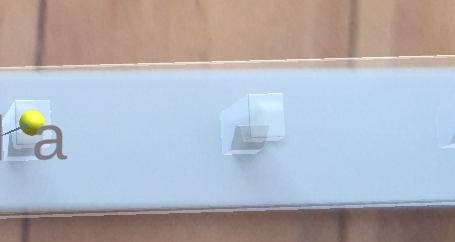
\includegraphics[width=.85\textwidth]{resources/implementation/ueberlagerung.png}
		\captionof{figure}{Digitaler Protottyp \\ Überlagerung des realen Produktes. Nicht optimal. \\Quelle: Eigene Darstellung}
		\label{fig:ueberlagerung}
	\end{minipage}%
	\begin{minipage}{.45\textwidth}
		\centering
		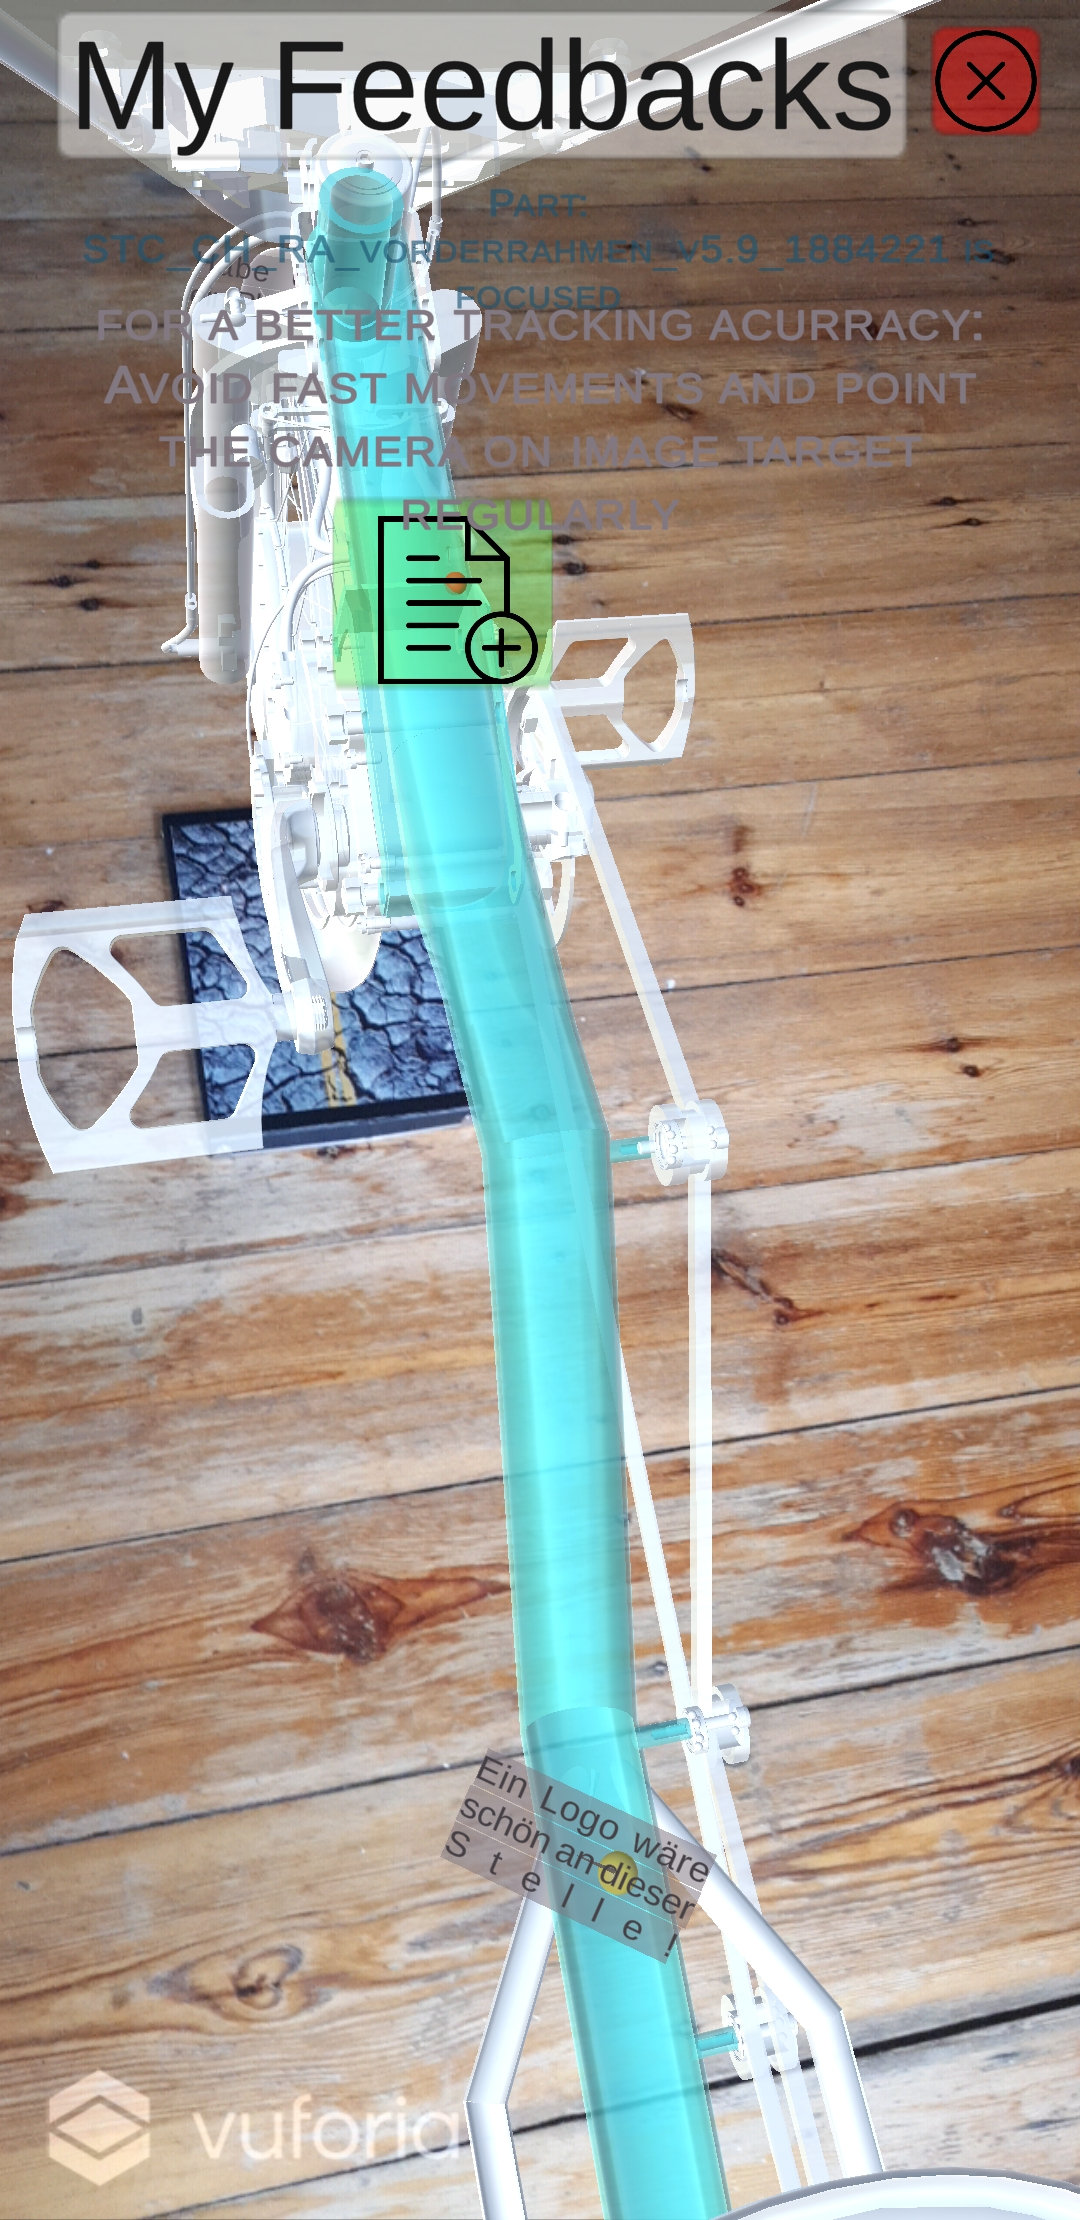
\includegraphics[width=.95\linewidth]{resources/implementation/annocreate.jpg}
		\captionof{figure}{Digitaler Protottyp \\ Auswahl einer Stelle am Produkt. \\Quelle: Eigene Darstellung}
		\label{fig:createdigi}
	\end{minipage}
\end{figure}

Für die Bearbeitung und Löschung von Feedback gibt es mit zwei unterschiedliche Darstellungsformen aus die, diese Aktionen durchgeführt werden können. 
Die Annotationsansicht welche auf Abbildung \ref{fig:annotationview} dargestellt ist sowie die Listenansicht welches auf Abbildung \ref{fig:listview} zu sehen ist. 

\begin{figure}[H]
	\label{tab:example}
	\centering
	\begin{minipage}{.45\textwidth}
		\centering
		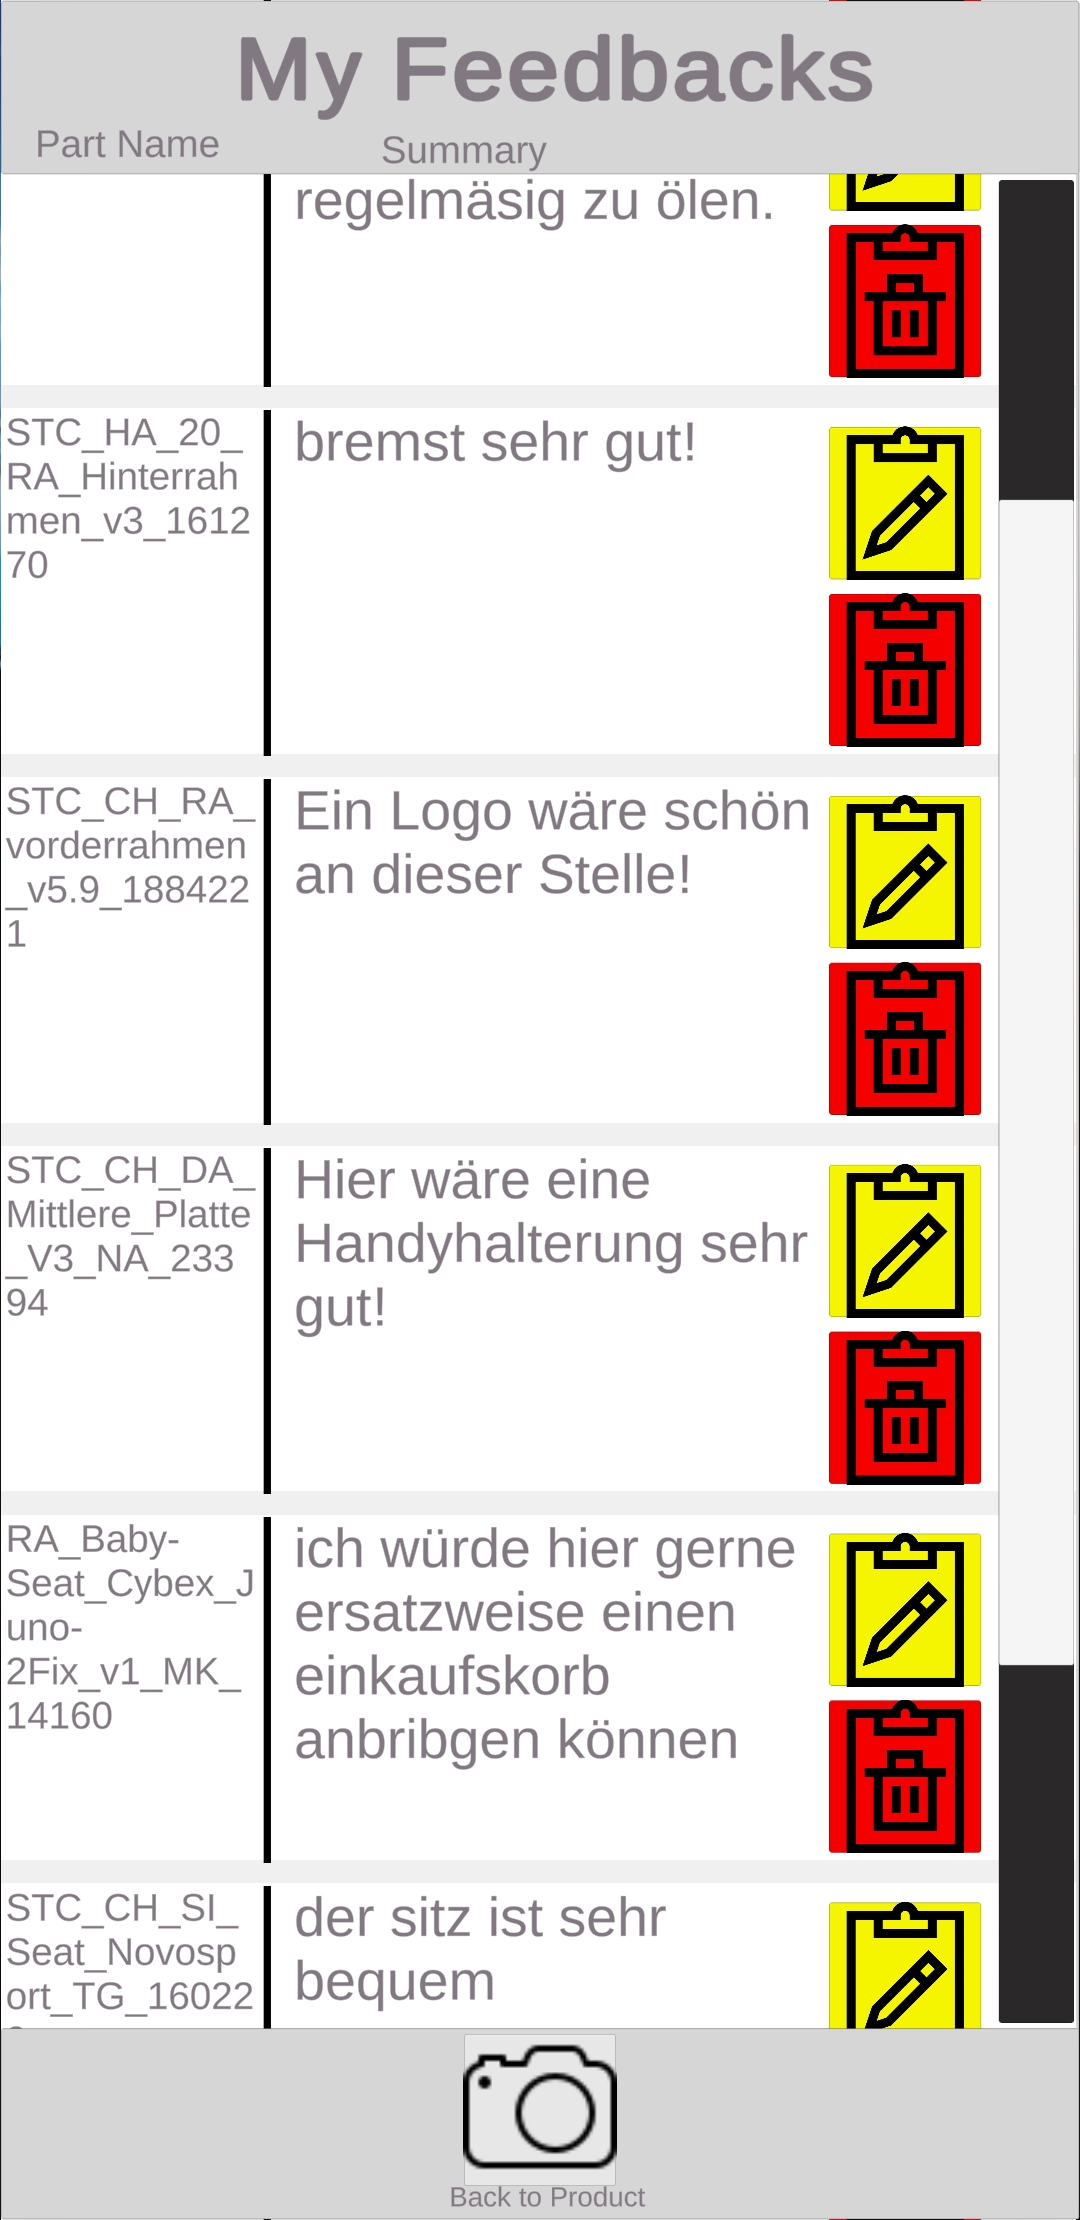
\includegraphics[width=.95\linewidth]{resources/implementation/listview.jpg}
		\captionof{figure}{Digitaler Protottyp \\Listenansicht \\Quelle: Eigene Darstellung}
		\label{fig:listview}
	\end{minipage}%
	\begin{minipage}{.45\textwidth}
		\centering
		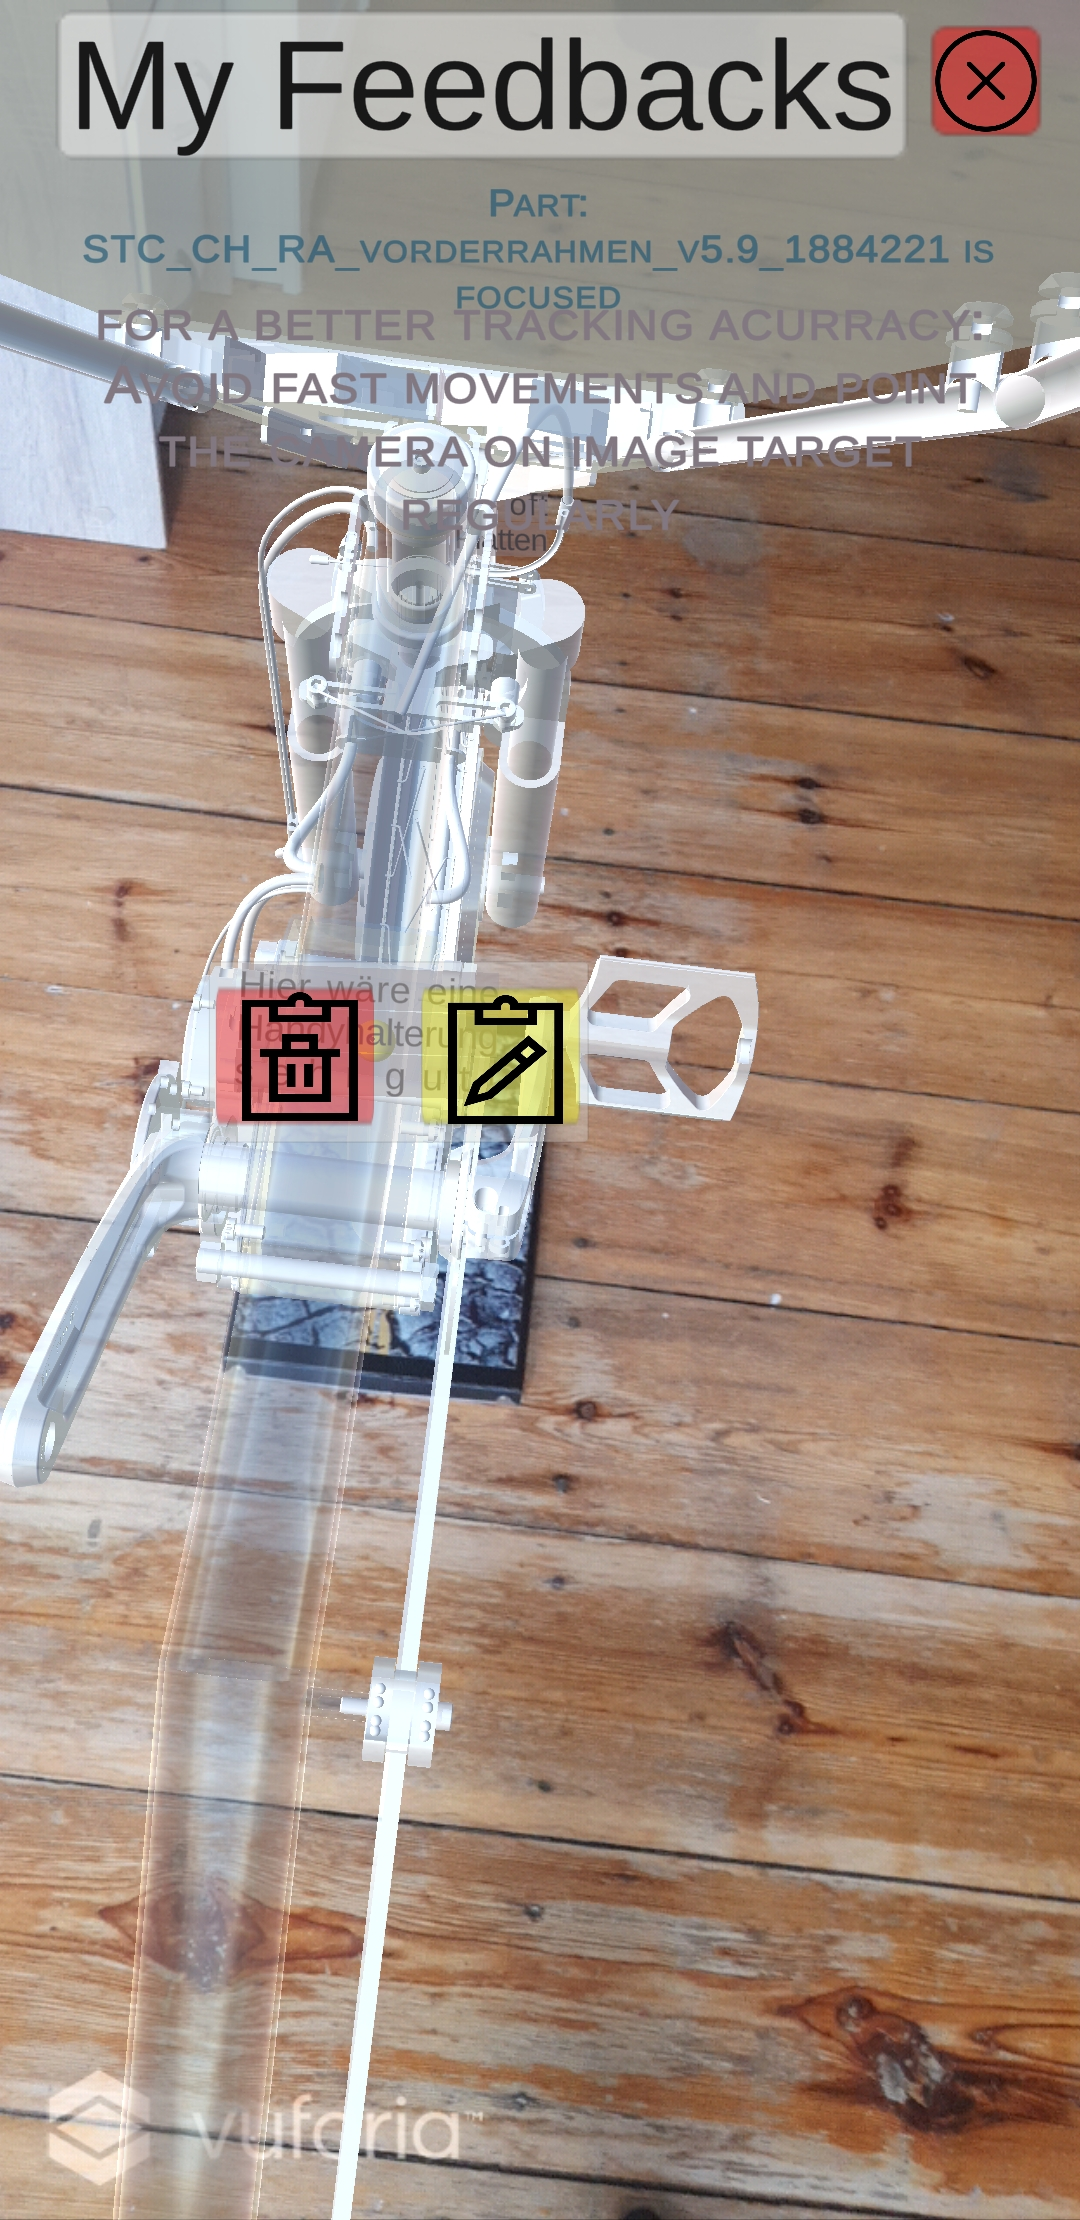
\includegraphics[width=.95\linewidth]{resources/implementation/annotationview.jpg}
		\captionof{figure}{Digitaler Protottyp \\ Annotationsansicht \\Quelle: Eigene Darstellung}
		\label{fig:annotationview}
	\end{minipage}
\end{figure}

Auf Abbildung \ref{fig:firstform} ist eine erste Version des Formular Ansicht für das Anlegen eines neuen Feedback zu sehen. 
Viele Elemente dieser Ansicht wurde von den Test Nutzern nicht verstanden. Insbesondere war ging nicht klar hervor wofür die einzelnen Kategorien 
stehen sowie was die Felder \textit{Impact} und \textit{Request Support} bewirken. Außerdem wurde festgestellt dass, das Formular keine Möglichkeit 
zur näheren Spezifizierung, ob auf die ausgewählte Stelle am Produkt oder das Produktteil Bezug genommen wird ermöglicht. 

So das Formular überarbeitet. Die überarbeitete Version ist auf Abbildung \ref{fig:secondform} zu sehen. Zu den Feldern welche nicht gut verstanden wurden,
wurden Beschreibungen hinzugefügt, welche diese näher beschreiben. Zudem wurden Icons verwendet welche die Bedeutung der Elemente verbildlichen. An einigen Stellen 
wurden Gestaltungsgesetze angewendet. Zum Beispiel wurde das  Gesetzt der Nähe verwendet und ähnliche Kategorien wie Design und New Usecase sowie Frage und Anleitung näher beieinander dargestellt. 
Des weiteren wurden die Buttons zum "Reset" zum Zurücksetzten der Eingaben sowie das Button zum zurückkehren in die AR Ansicht mit einem Abstand zum "Submit" Button, für die Bestätigung der Eingaben 
dargesetllt. Das Gesetzt der Unentschlossenheit wurde angewendet um zu zeigen dass die zwei Kontrollkästchen für die Auswahl ob Bezug auf eine bestimmte Stelle am Produkt genommen wir oder auf ein 
Produktteil zusammen gehören. 

\begin{figure}[H]
	\label{tab:example}
	\centering
	\begin{minipage}{.45\textwidth}
		\centering
		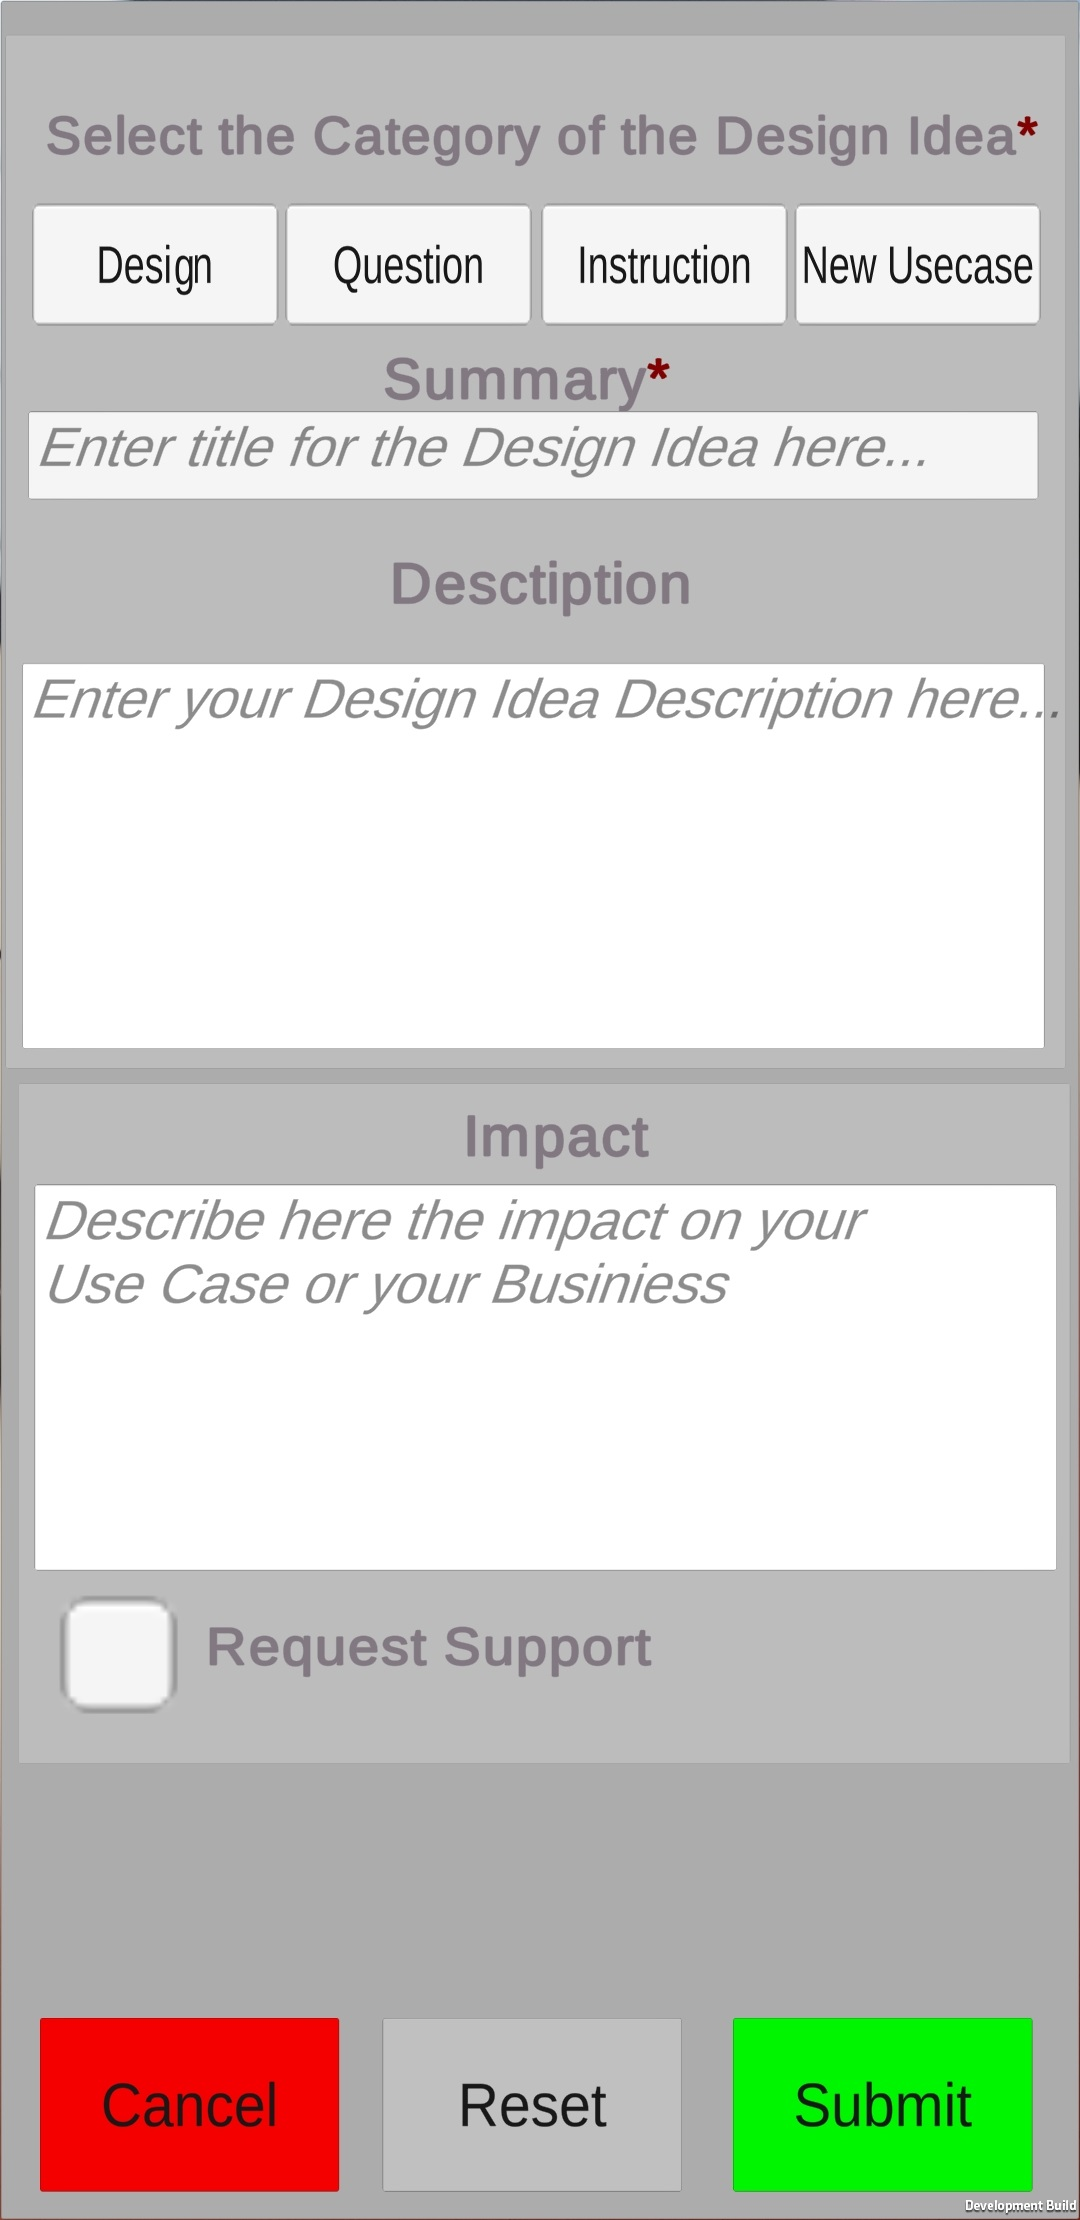
\includegraphics[width=.95\linewidth]{resources/implementation/firstform.jpg}
		\captionof{figure}{Digitaler Protottyp \\Formualransicht Version 1\\Quelle: Eigene Darstellung}
		\label{fig:firstform}
	\end{minipage}%
	\begin{minipage}{.45\textwidth}
		\centering
		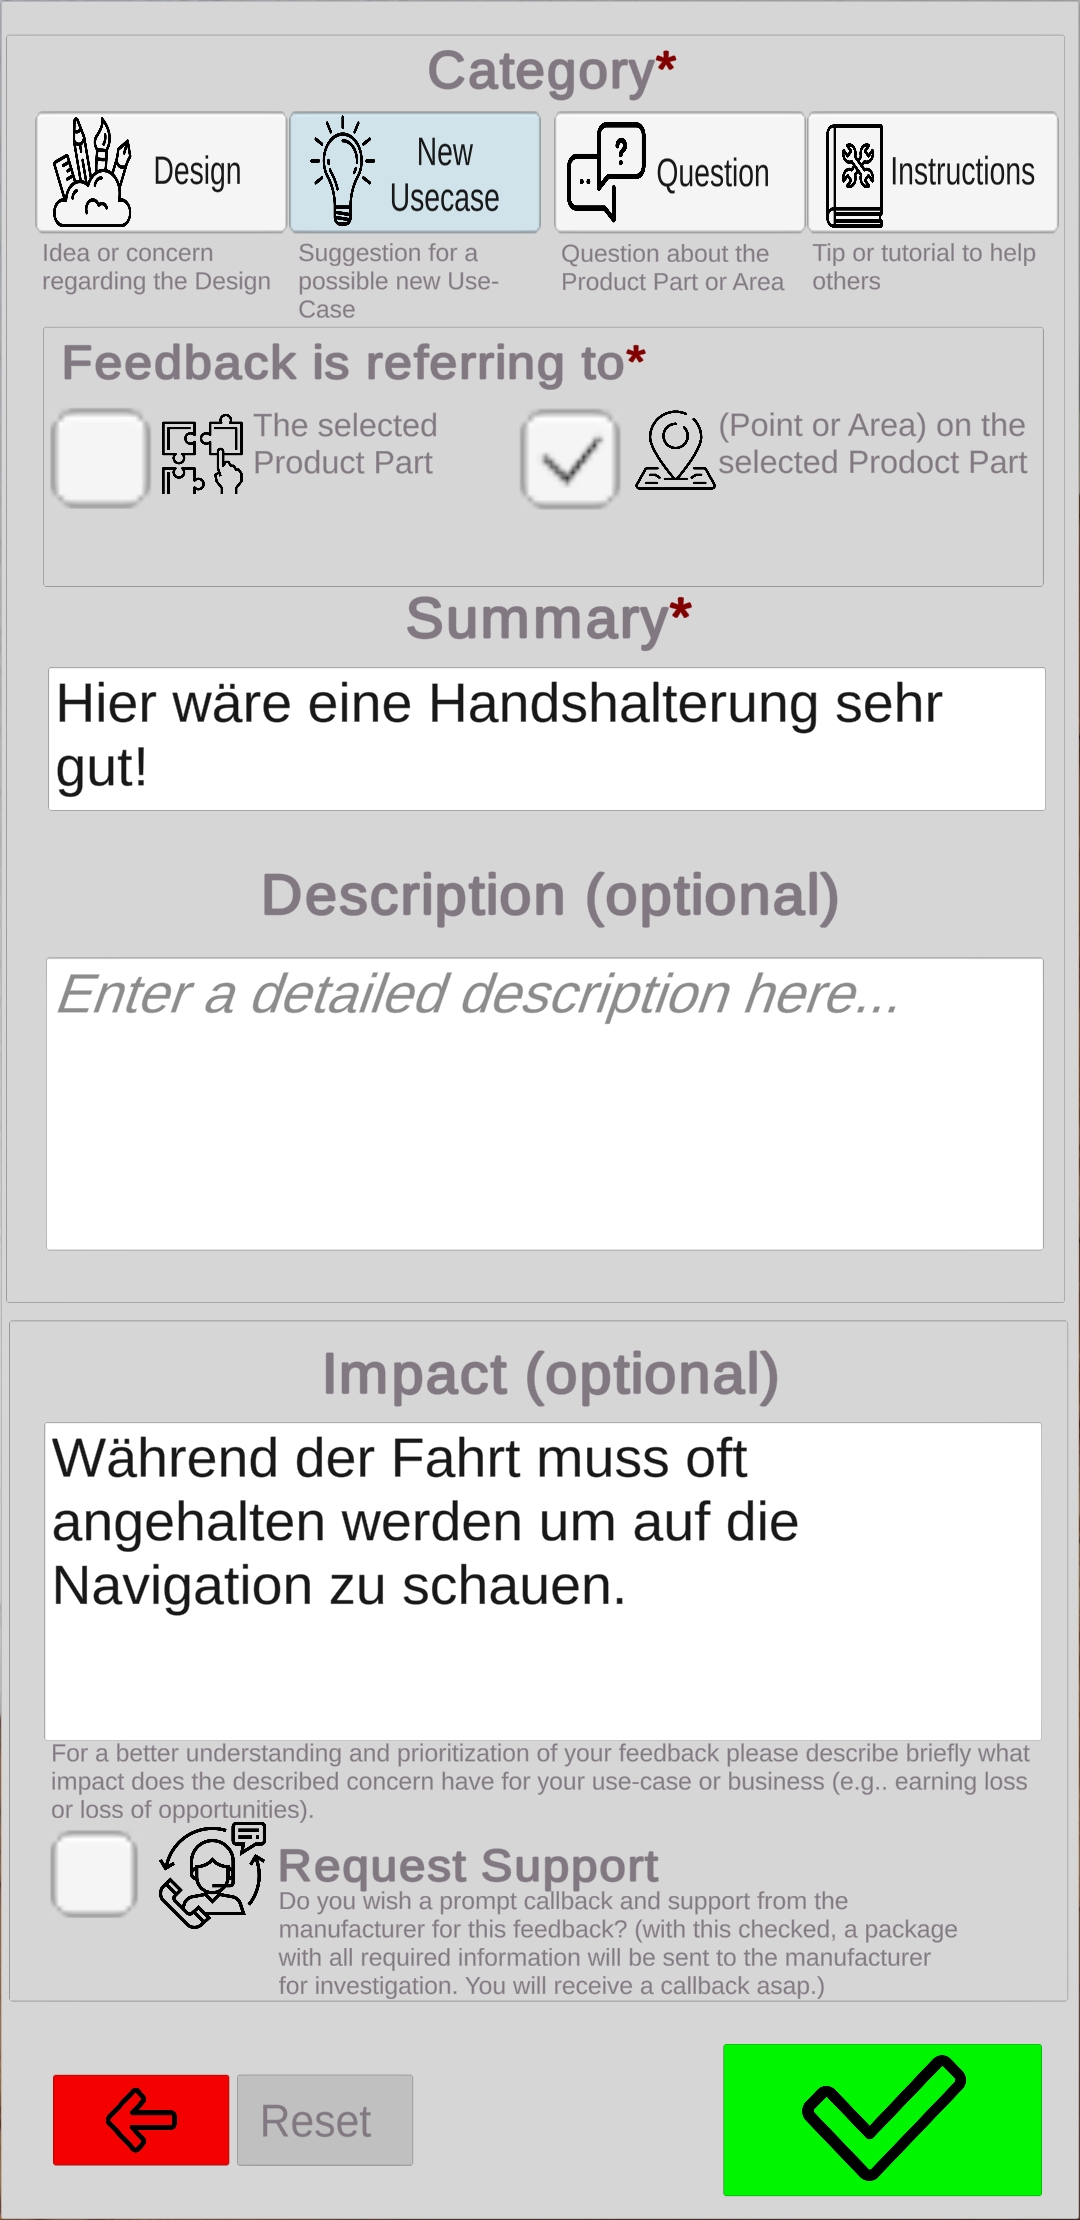
\includegraphics[width=.95\linewidth]{resources/implementation/secondform.jpg}
		\captionof{figure}{Digitaler Protottyp \\ Formularansicht Version 2\\Quelle: Eigene Darstellung}
		\label{fig:secondform}
	\end{minipage}
\end{figure}

\section{Zeiterfassung für die Studie}

Für die Zeiterfassung der durchzuführenden Aktionen in der Studie wurde beschlossen für jede durchgeführte Aktion
jeweils in der Start Methode der SelektionManager Klasse die Zeitmessung zu starten und bei der jeweiligen Aktion zu stoppen.
Die Start Methode wird wird nur einmal im Lebenszyklus des Skriptes ausgeführt und wird vor der ersten Ausführung der Update Funktion ausgeführt welcher in jeder Frame ausgeführt wird. \cite{Unity}

Für die Erstellung und Bearbeitung wurde die Zeit jeweils in der Methode gestoppt in welcher die Szene für die Formular Ansicht \ref{fig:secondform}
geöffnet wurde. Für das Löschen wurde die Zeit in der Methode gestoppt in welcher die Lösch-Methode des StorageManagers aufgerufen wurde. 

Der Datentyp (Sihe Abbildung \ref{img:entitytype}) für ein Feedback wurde um drei weitere Felder ergänzt in welcher die Zeiten für die jeweiligen Aktionen festgehalten wurden. In drei neuen Felder vom Datentyp Integer wurde jeweils die Zeit
in Millisekunden gespeichert die benötigt wurde um in das Formular zum Erstellen bzw. zum Bearbeiten zu gelangen sowie die Zeit die die benötigt wurde um ein Feedback zu löschen. 
Die Werde wurden in eine XML Datei gespeichert wenn die Applikation beendet wurde. 

Es wurde vorausgesetzt dass nach jeder Aufgabe die Anwendung neugestartet werden musste damit die Startzeit, da diese in der Start Methode des SelektionManager Klasse beginnt für die neue Aufgabe zurückgesetzt wird. 
Sicherlich hätte dies eleganter gelöst werden können, doch diese Methode wurde getestet und als sicher empfunden. Auf Grund des Zeitmangels wurde die Zeitmessung bei dieser Methode belassen.
